
\begin{correction}  \;
\begin{enumerate}
%--------------------------------------------------
\item \textbf{R\'esolution de $\mathbf{\sin{x}-\cos{x}=\ddp\frac{\sqrt{6}}{2}}$:}
On reconna\^{i}t la forme $a\cos{(x)}+b\sin{(x)}$, on applique donc la m\'ethode associ\'ee. On obtient alors
$$\begin{array}{lll} \sin{x}-\cos{x}=\ddp\frac{\sqrt{6}}{2} &\Leftrightarrow &\sqrt{2}\left( -\ddp\frac{1}{\sqrt{2}}\cos{(x)}+\ddp\frac{1}{\sqrt{2}}\sin{(x)}  \right)=\ddp\frac{\sqrt{3}\sqrt{2}}{2}\Leftrightarrow \cos{\left( x-\ddp\frac{3\pi}{4} \right)}=\ddp\frac{\sqrt{3}}{2}\vsec\\
&\Leftrightarrow& \left\lbrace\begin{array}{lllll} \exists k\in\Z,& x-\ddp\frac{3\pi}{4} &=&  \ddp\frac{\pi}{6}+2k\pi \vsec\\ \exists k\in\Z,& x-\ddp\frac{3\pi}{4} &=&  -\ddp\frac{\pi}{6}+2k\pi\end{array}\right. \end{array}$$ 
\begin{minipage}[c]{0.45\linewidth}
On obtient ainsi:
\begin{itemize}
\item[$\bullet$] Sur $\R$ : 
$$\fbox{$\mathcal{S}_\R=\left\lbrace \ddp\frac{11\pi}{12}+2k\pi,\ k\in\Z  \right\rbrace\cup \left\lbrace \ddp\frac{7\pi}{12}+2k\pi,\ k\in\Z  \right\rbrace.$}$$
 \item[$\bullet$] Sur $\lbrack 0,2\pi\lbrack$ comme sur $\rbrack -\pi,\pi\rbrack$ : 
 $$\fbox{$\mathcal{S}_{[0,2\pi[}=\mathcal{S}_{]-\pi,\pi]}= \left\lbrace \ddp\frac{7\pi}{12},\ddp\frac{11\pi}{12} \right \rbrace.$}$$
\end{itemize}
\end{minipage}
\quad

\begin{center}
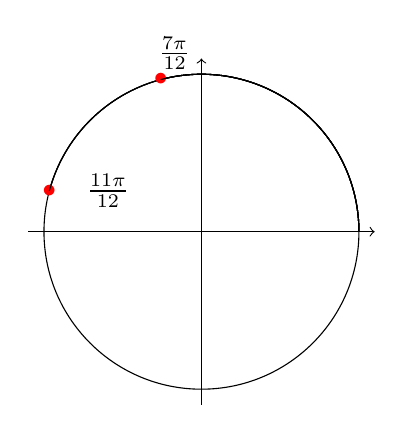
\begin{tikzpicture}[scale=2]
%Axes
\draw [->] (-1.1,0) -- (1.1,0);
\draw [->] (0,-1.1) -- (0,1.1);
%Cercle
\draw (0,0) circle (1);
%Points
\draw (1,0) arc (0:165:1) node [red] {$\bullet$};
\draw (1,0) arc (0:165:1) node[right] {$\quad \ddp \frac{11\pi}{12}$} ;
\draw (1,0) arc (0:105:1) node [red] {$\bullet$};
\draw (1,0) arc (0:105:1) node[above] {$\quad \ddp \frac{7\pi}{12}$} ;
\end{tikzpicture}
\end{center}

%--------------------------------------------------
\item  \textbf{R\'esolution de $\mathbf{ -\sqrt{3}\sin{x}+\cos{x}=\sqrt{2}}$:}
M\^{e}me m\'ethode que dans l'exemple pr\'ec\'edent. On obtient ainsi
\begin{itemize}
\item[$\bullet$] Sur $\R$ : 
$$\fbox{$\mathcal{S}_\R=\left\lbrace \ddp-\frac{7\pi}{12}+2k\pi,\ k\in\Z  \right\rbrace\cup \left\lbrace - \ddp\frac{\pi}{12}+2k\pi,\ k\in\Z  \right\rbrace .$}$$
\end{itemize}
\begin{minipage}[c]{0.45\linewidth}
\begin{itemize}
\item[$\bullet$] Sur $\lbrack 0,2\pi\lbrack$ : 
$$\fbox{$\mathcal{S}=\left\lbrace \ddp\frac{17\pi}{12},\ddp\frac{23\pi}{12} \right \rbrace.$}$$
\item[$\bullet$] Sur $\lbrack -\pi,\pi\lbrack$ :
$$\fbox{$\mathcal{S}=\left\lbrace -\ddp\frac{\pi}{12},-\ddp\frac{7\pi}{12} \right \rbrace.$}$$
\end{itemize}
\end{minipage}
\quad

\begin{center}
\begin{tikzpicture}[scale=2]
%Axes
\draw [->] (-1.1,0) -- (1.1,0);
\draw [->] (0,-1.1) -- (0,1.1);
%Cercle
\draw (0,0) circle (1);
%Points
\draw (1,0) arc (0:255:1) node [red] {$\bullet$};
\draw (1,0) arc (0:255:1) node[below] {$\quad \ddp - \frac{7\pi}{12}$} ;
\draw (1,0) arc (0:-15:1) node [red] {$\bullet$};
\draw (1,0) arc (0:-15:1) node[right] {$\quad \ddp - \frac{\pi}{12}$} ;
\end{tikzpicture}
\end{center}

%--------------------------------------------------
\item  \textbf{R\'esolution de $\mathbf{ \sin{x}+\ddp\frac{1}{\sqrt{3}}\cos{x}=0 }$:}
M\^{e}me m\'ethode que dans l'exemple pr\'ec\'edent. On a: 
$$\sin{x}+\ddp\frac{1}{\sqrt{3}}\cos{x}=0 \Leftrightarrow \cos{\left(  x-\ddp\frac{\pi}{3}\right)=0}\Leftrightarrow \exists k\in\Z,\ x-\ddp\frac{\pi}{3}=\ddp\frac{\pi}{2}+k\pi.$$ 
On obtient ainsi:\\
\begin{minipage}[c]{0.45\linewidth}
\begin{itemize}
\item[$\bullet$] Sur $\R$: \fbox{$\mathcal{S}=\left\lbrace \ddp\frac{5\pi}{6}+k\pi,\ k\in\Z  \right\rbrace.$}
\item[$\bullet$] Sur $\lbrack 0,2\pi\lbrack$: \fbox{$\mathcal{S}=\left\lbrace \ddp\frac{5\pi}{6},\ddp\frac{11\pi}{6} \right \rbrace.$}
\item[$\bullet$]  Sur $\lbrack -\pi,\pi\lbrack$: \fbox{$\mathcal{S}=\left\lbrace -\ddp\frac{\pi}{6},\ddp\frac{5\pi}{6} \right \rbrace.$}
\end{itemize}
\end{minipage}
\quad
-
\begin{center}
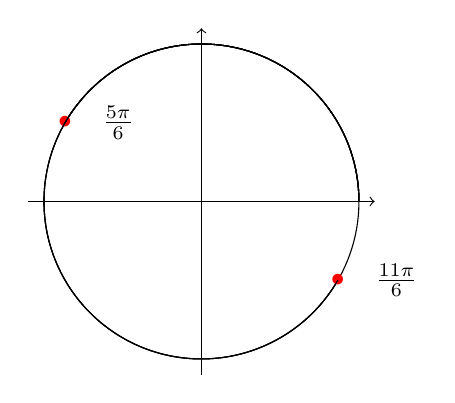
\begin{tikzpicture}[scale=2]
%Axes
\draw [->] (-1.1,0) -- (1.1,0);
\draw [->] (0,-1.1) -- (0,1.1);
%Cercle
\draw (0,0) circle (1);
%Points
\draw (1,0) arc (0:150:1) node [red] {$\bullet$};
\draw (1,0) arc (0:150:1) node[right] {$\quad \ddp \frac{5\pi}{6}$} ;
\draw (1,0) arc (0:330:1) node [red] {$\bullet$};
\draw (1,0) arc (0:330:1) node[right] {$\quad \ddp \frac{11\pi}{6}$} ;
\end{tikzpicture}
\end{center}

%---------------------------------------------------
\item \textbf{R\'esolution de $\mathbf{ \cos{(2x)}+\sqrt{3}\sin{(2x)}=\sqrt{2}  }$:}
Quitte \`{a} poser $X=2x$, l'\'egalit\'e est de type $a\cos{(X)}+b\sin{(X)}=c$, on applique donc la m\'ethode du cours. On se ram\`ene ainsi \`a l'\'equation fondamentale suivante:   $\cos{(X-\ddp\frac{\pi}{3})}=\ddp\frac{\sqrt{2}}{2}\Leftrightarrow \cos{(2x-\ddp\frac{\pi}{3})}=\ddp\frac{\sqrt{2}}{2}.$
Ainsi,
$$
\cos{(2x)}+\sqrt{3}\sin{(2x)}=\sqrt{2}\Leftrightarrow 
\left\lbrace
\begin{array}{l}
\exists k\in\Z,\ 2x-\ddp\frac{\pi}{3}=\ddp\frac{\pi}{4}+2k\pi\vsec\\
\hbox{ou}\vsec\\
\exists k\in\Z,\ 2x-\ddp\frac{\pi}{3}=-\ddp\frac{\pi}{4}+2k\pi.
\end{array}\right.
$$
On obtient ainsi:
\begin{itemize}
\item[$\bullet$] Sur $\R$ : \fbox{$\mathcal{S}=\left\lbrace x\in\R;\   \exists k\in\Z,\ x=\ddp\frac{7\pi}{24}+k\pi\right\rbrace\cup\left\lbrace x\in\R;\   \exists k\in\Z,\ x=\ddp\frac{\pi}{24}+k\pi\right\rbrace .$}
\end{itemize}
\begin{minipage}[c]{0.45\textwidth}
\begin{itemize}
\item[$\bullet$] Sur $\lbrack 0,2\pi\lbrack$ : \conclusion{$\mathcal{S}=\left\lbrace \ddp\frac{\pi}{24},\ddp\frac{7\pi}{24},\ddp\frac{25\pi}{24},\ddp\frac{31\pi}{24}   \right \rbrace.$}
\item[$\bullet$] Sur $]-\pi,\pi]$ : 

\conclusion{$\mathcal{S}=\left\lbrace -\ddp\frac{23\pi}{24},-\ddp\frac{17\pi}{24},\ddp\frac{\pi}{24},\ddp\frac{7\pi}{24}     \right\rbrace.$}
\end{itemize}
\end{minipage}


\begin{center}
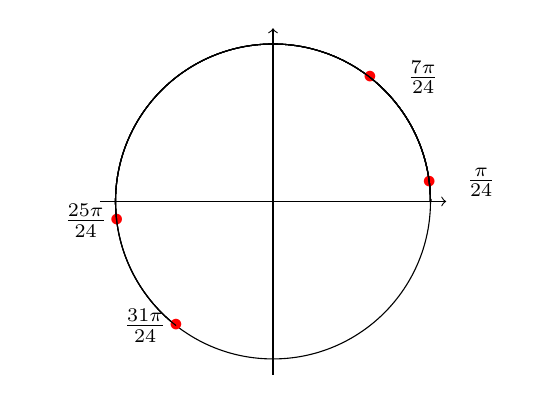
\begin{tikzpicture}[scale=2]
%Axes
\draw [->] (-1.1,0) -- (1.1,0);
\draw [->] (0,-1.1) -- (0,1.1);
%Cercle
\draw (0,0) circle (1);
%Points
\draw (1,0) arc (0:7:1) node [red] {$\bullet$};
\draw (1,0) arc (0:7:1) node[right] {$\quad \ddp \frac{\pi}{24}$} ;
\draw (1,0) arc (0:187:1) node [red] {$\bullet$};
\draw (1,0) arc (0:187:1) node[left] {$\quad \ddp \frac{25\pi}{24}$} ;
\draw (1,0) arc (0:52:1) node [red] {$\bullet$};
\draw (1,0) arc (0:52:1) node[right] {$\quad \ddp \frac{7\pi}{24}$} ;
\draw (1,0) arc (0:232:1) node [red] {$\bullet$};
\draw (1,0) arc (0:232:1) node[left] {$\quad \ddp \frac{31\pi}{24}$} ;
\end{tikzpicture}
\end{center}

\end{enumerate}
\end{correction}